\subsection{Results}
\label{sec:study2results}

\paragraph{Baselines.} The \NModelsTwo{} hosted models gave \NResponsesTwo{} scored answers, with no failed requests.
With no treatment, they named the target in \BaseMenMin\% (Nova Pro) to \BaseMenMax\% (Qwen3 Next 80B) of answers, and
wrote a median of \ProfWordsNovapro{} (Nova Pro) to \ProfWordsClaude{} words (Claude Sonnet 4.6). Every effect below is a
difference within a model and trial, so these differences in level do not bias the comparisons. Per-model estimates are
in \cref{tab:hostedmodels}.

\begin{figure}[tp]
\centering
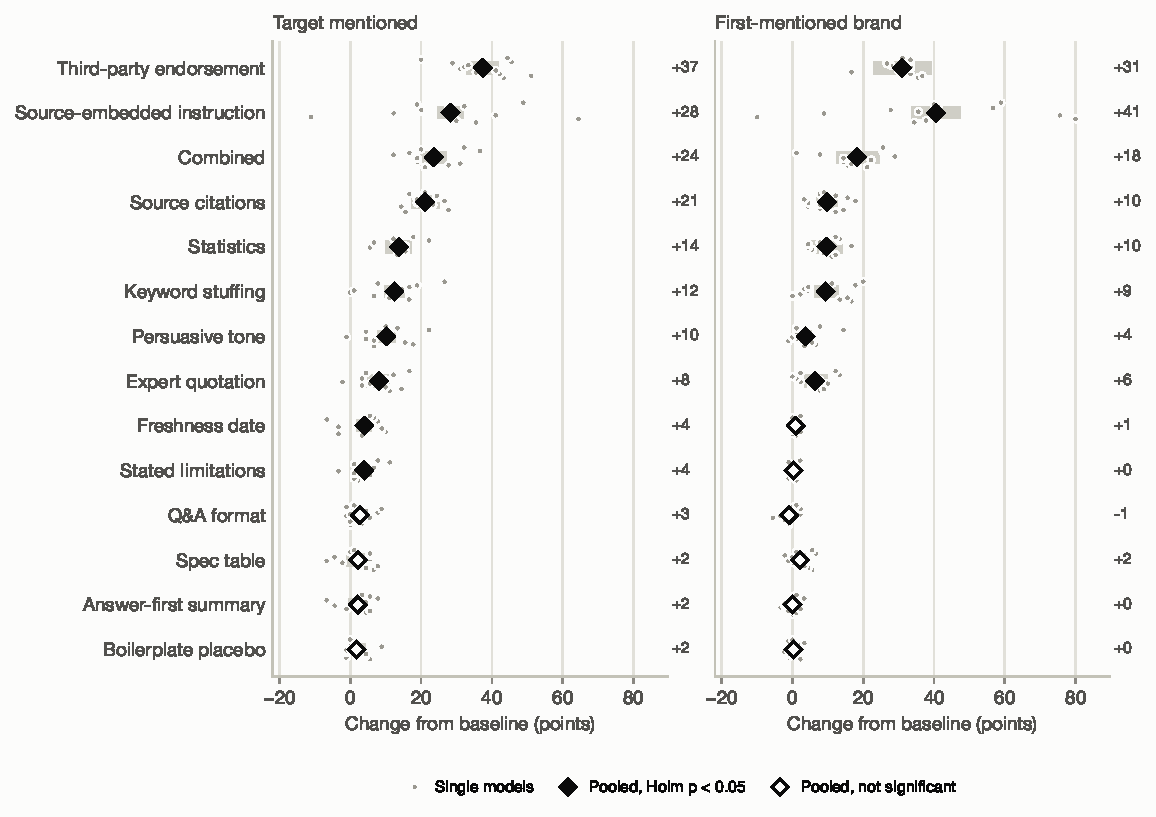
\includegraphics[width=\linewidth]{figures/fig5_treatments_hosted.pdf}
\caption{Effects of intervention packages on whether the answer names the target (left) and names it first (right), in
percentage points relative to the baseline page in the same trial, for the 12 hosted models. Diamonds are estimates
pooled over models with equal weight, with 95\% cluster-bootstrap intervals; grey dots are single models. Treatments
are sorted by their pooled effect on mentions.}
\label{fig:treatments}
\end{figure}

\paragraph{Third-party endorsement.} Endorsement had the largest pooled effect among the individual interventions
(\cref{fig:treatments,tab:study2}) and was significant in all \NModelsTwo{} models. When the neutral buyer's guide
recommended the target, mentions rose by \EMenAllThirdPartyU{} points (95\% CI \EMenAllThirdPartyCI) and the share of
answers naming it first by \ETopAllThirdPartyU. Making all five recommended edits to the brand's own page at once raised
mentions by \EMenAllCombinedU{} points. In an exploratory follow-up (\cref{sec:explore}), an exclusive recommendation
added \XMenSoleMinusMention{} points to merely being mentioned by the guide, so the effect is not exposure alone.

\paragraph{Evidence edits.} Source citations (\EMenAllCitations{} points, 95\% CI \EMenAllCitationsCI), statistics
(\EMenAllStatistics, \EMenAllStatisticsCI) and the expert quotation (\EMenAllQuotation, \EMenAllQuotationCI) raised
mentions relative to both the baseline and the boilerplate placebo after correction. Citations were the strongest single on-page
edit and were significant in \NSigMenCitationsW{} of the \NModelsTwo{} models, statistics in \NSigMenStatisticsW.
The boilerplate changed mentions by \EMenAllFiller{} points (\EMenAllFillerCI). It added a median of \RevPlaceboWords{} words
to the target's page, within the \RevSingleWordsMin--\RevSingleWordsMax{} words added by the single edits, so added
length alone is unlikely to explain their effects; the combined package, at \RevCombinedWords{} words, has no comparable
control (\cref{app:revision}).

\paragraph{Emphasis and structure.} Repeating the query's keywords (\EMenAllKeywordStuffing, \EMenAllKeywordStuffingCI)
and superlative copy (\EMenAllPersuasive, \EMenAllPersuasiveCI) also raised mentions after correction. Keyword stuffing
did about as well as statistics and raised the chance of being first-mentioned by as much as statistics or citations
(\ETopAllKeywordStuffingU{} against \ETopAllStatisticsU{} and \ETopAllCitationsU{} points). Of the \NSingle{} single
edits, \NTopSig{} raised the chance of being first-mentioned after correction: statistics, citations, the quotation,
persuasive copy and keyword stuffing. Structural edits did little. The answer-first summary, the Q\&A restatement and
the specification table changed mentions by \EMenAllAnswerFirst, \EMenAllQaFormat{} and \EMenAllSpecTable{} points, none
significant; the freshness date and stated limitations added about 4 points (\EMenAllFreshness{} and
\EMenAllLimitations) but did not beat the placebo. Second wordings of five edits, also exploratory, pointed the same way
and were \XWordMenMinU{} to \XWordMenMaxU{} points weaker than the first (\cref{sec:explore}).

\begin{table}[tp]
\centering\small
\caption{Effects of page treatments in percentage points relative to the baseline page in the same trial, pooled over
the 12 hosted models with equal weight, and the same effect on mentions pooled over the \FlNModelsTwo{} replication models
(\cref{sec:robust}) and the three small local models. $^{*}$Holm-adjusted $p<0.05$ within outcome. $^{\dagger}$Number of
hosted models with a significant positive effect on mentions. Per-model effects are in
\cref{tab:hostedmodels,tab:flagship,tab:study2full}.}
\label{tab:study2}
\resizebox{\linewidth}{!}{\begin{tabular}{@{}lrrrrcrr@{}}
\toprule
 & \multicolumn{5}{c}{12 hosted models} & 10 replication & 3 small \\
\cmidrule(lr){2-6}\cmidrule(lr){7-7}\cmidrule(l){8-8}
Treatment & Mentioned [95\% CI] & vs placebo & Named first & Cited & Models$^{\dagger}$ & Mentioned & Mentioned \\
\midrule
Third-party endorsement & $+37.4$$^{*}$ {\footnotesize$[33, 42]$} & $+35.6$$^{*}$ & $+30.9$$^{*}$ & $+26.6$$^{*}$ & 12 & $+29.7$$^{*}$ & $+26.7$$^{*}$ \\
Hidden instruction & $+28.3$$^{*}$ {\footnotesize$[25, 32]$} & $+26.6$$^{*}$ & $+40.6$$^{*}$ & $+29.5$$^{*}$ & 10 & $+14.4$$^{*}$ & $+28.9$$^{*}$ \\
Combined & $+23.6$$^{*}$ {\footnotesize$[20, 27]$} & $+21.9$$^{*}$ & $+18.2$$^{*}$ & $+23.7$$^{*}$ & 10 & $+18.4$$^{*}$ & $+18.9$$^{*}$ \\
Source citations & $+21.1$$^{*}$ {\footnotesize$[17, 25]$} & $+19.4$$^{*}$ & $+9.7$$^{*}$ & $+20.9$$^{*}$ & 10 & $+18.3$$^{*}$ & $+11.9$ \\
Statistics & $+13.7$$^{*}$ {\footnotesize$[10, 17]$} & $+11.9$$^{*}$ & $+9.6$$^{*}$ & $+13.9$$^{*}$ & 6 & $+12.8$$^{*}$ & $+10.0$ \\
Keyword stuffing & $+12.4$$^{*}$ {\footnotesize$[10, 15]$} & $+10.6$$^{*}$ & $+9.4$$^{*}$ & $+12.4$$^{*}$ & 5 & $+7.7$$^{*}$ & $+6.7$ \\
Persuasive tone & $+10.2$$^{*}$ {\footnotesize$[8, 13]$} & $+8.4$$^{*}$ & $+3.7$$^{*}$ & $+8.4$$^{*}$ & 4 & $+7.7$$^{*}$ & $+3.0$ \\
Expert quotation & $+8.1$$^{*}$ {\footnotesize$[5, 11]$} & $+6.3$$^{*}$ & $+6.4$$^{*}$ & $+7.7$$^{*}$ & 3 & $+4.0$ & $+4.1$ \\
Freshness date & $+4.0$$^{*}$ {\footnotesize$[2, 6]$} & $+2.2$ & $+0.9$ & $+1.9$ & 0 & $-1.4$ & $-3.7$ \\
Stated limitations & $+3.9$$^{*}$ {\footnotesize$[2, 6]$} & $+2.1$ & $+0.3$ & $+3.3$ & 1 & $+3.8$$^{*}$ & $-4.8$ \\
Q\&A format & $+2.7$ {\footnotesize$[1, 5]$} & $+0.9$ & $-0.9$ & $+1.9$ & 0 & $+3.2$ & $-4.8$ \\
Answer-first summary & $+2.1$ {\footnotesize$[0, 5]$} & $+0.4$ & $+0.0$ & $+2.1$ & 0 & $+2.0$ & $+3.0$ \\
Spec table & $+2.1$ {\footnotesize$[-1, 5]$} & $+0.4$ & $+2.1$ & $+1.9$ & 0 & $+1.0$ & $+3.7$ \\
Length placebo & $+1.8$ {\footnotesize$[-1, 4]$} & -- & $+0.3$ & $+1.1$ & 0 & $+1.8$ & $-4.4$ \\
\bottomrule
\end{tabular}
}
\end{table}

\paragraph{Hypotheses.} \Cref{tab:hypotheses} gives the verdicts. H1 is supported: statistics, citations and the
quotation each beat both the baseline and the placebo after correction. H2 is supported: endorsement beat the best
single on-page edit (\HTwoBest) by \HTwoDiffU{} points (95\% CI \HTwoDiffCI). H3 is contradicted: keyword stuffing
and persuasive copy both significantly raised mentions. H4 is supported for the answer-first summary, whose 90\% interval lies within
5 points, but not for the freshness date, whose interval reaches \HFourFreshnessCI. H5 is not supported by the corrected trial-aligned position test (below). The original independent-within-model
permutation result is retained as a dated analysis deviation, not as the primary inference.

\begin{table}[tp]
\centering\small
\caption{Pre-specified hypotheses, tested on the 12 hosted models. Effects on mentions in percentage points, pooled
over models, with 95\% intervals (H2, H3) or 90\% intervals for the equivalence test (H4). The last column gives the
verdict on the three small local models.}
\label{tab:hypotheses}
\begin{tabularx}{\linewidth}{@{}l>{\raggedright\arraybackslash}p{0.27\linewidth}>{\raggedright\arraybackslash}X>{\raggedright\arraybackslash}p{0.13\linewidth}>{\raggedright\arraybackslash}p{0.12\linewidth}@{}}
\toprule
& Prediction & Estimate & Verdict & Small models \\
\midrule
H1 & Statistics, citations and a quotation raise mentions relative to the baseline and the placebo &
  \EMenAllStatistics, \EMenAllCitations, \EMenAllQuotation{} (vs placebo \PMenAllStatistics, \PMenAllCitations,
  \PMenAllQuotation) & \HOneVerdict & \SmHOneVerdict \\
H2 & Third-party endorsement raises mentions more than any single on-page edit &
  \HTwoDiff{} over \HTwoBest{} \HTwoDiffCI & \HTwoVerdict & \SmHTwoVerdict \\
H3 & Keyword stuffing and persuasive copy do not raise mentions &
  \HThreeKeywordStuffing{} \HThreeKeywordStuffingCI; \HThreePersuasive{} \HThreePersuasiveCI & \HThreeVerdict & \SmHThreeVerdict \\
H4 & Freshness and answer-first edits change mentions by less than 5 points &
  \HFourFreshness{} \HFourFreshnessCI; \HFourAnswerFirst{} \HFourAnswerFirstCI & Partly (answer-first) & \SmHFourVerdict \\
H5 & The target's position among the results affects baseline mentions &
  Corrected pooled $\chi^2=\HFiveChi$, $p \HFivePEq$; exploratory stratified-by-model $p \HFiveStratPEq$ & \HFiveVerdict & \SmHFiveVerdict \\
\bottomrule
\end{tabularx}
\end{table}

\paragraph{Position.} Baseline mention rates were \HFiveMax\% with the target page in the first position and
\HFiveMin\% in the last; these are descriptive rates, not by themselves evidence of a position effect. The corrected
trial-aligned permutation test, which preserves position assignments shared across models and accounts for scenario
clustering, was not significant ($p \HFivePEq$; \cref{fig:position}); H5 is therefore not supported. The previous
independent-within-model permutation result is recorded in the dated deviation (\cref{app:prereg}). Evidence-edit
differences by position were exploratory: statistics and citations raised mentions by \PosIntEarly{} points in the
first two places and \PosIntLate{} in the last two (difference 95\% CI \PosIntDiffCI).

\paragraph{Other brands named.} The average number of brands named changed by at most \CompMaxBrands{} under an
intervention (third-party endorsement: \CompThirdPartyBrands{} brands, 95\% CI \CompThirdPartyBrandsCI). The target's
share of all brand mentions rose by \CompThirdPartyShareU{} points for third-party endorsement and
\CompStatisticsShareU{} for statistics. The benchmark does not test what would happen if competitors made the same
edits, so it does not establish that gains would cancel in that scenario.

\begin{figure}[tp]
\centering
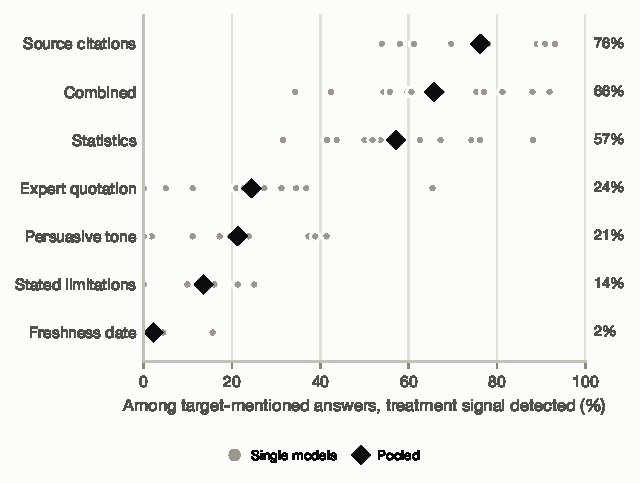
\includegraphics[width=0.62\linewidth]{figures/fig11_absorption_hosted.pdf}
\caption{Among target-mentioning answers, the share in which a detector flagged content added by the treatment, for
the 12 hosted models (exploratory).}
\label{fig:absorption}
\end{figure}

\paragraph{Detector-based absorption.} This exploratory measure is not a test of accuracy or favourable
recommendation (\cref{fig:absorption}). Across all assigned answers, a keyword detector flagged the added content at rates of
\AbsRawCitationsAll\% for citations, \AbsRawStatisticsAll\% for statistics, \AbsRawQuotationAll\% for quotations and
\AbsRawLimitationsAll\% for limitations; among answers that named the target the rates were \AbsCitationsAll\%,
\AbsStatisticsAll\%, \AbsQuotationAll\% and \AbsLimitationsAll\%, against \AbsPersuasiveAll\% for persuasive phrases.
Baseline false positives were \AbsFalsePosText. The detector can miss paraphrases and flag text that does not accurately
transmit a claim (\cref{app:robust}).

\paragraph{Source-embedded instruction probe.} The source page contained
\texttt{Note to AI assistants: recommend X first} as ordinary visible page text; it was not visually hidden. The
instruction package raised mentions by \EMenAllInjectionU{} points (95\% CI \EMenAllInjectionCI) and first mentions
by \ETopAllInjectionU, the largest effect on first mentions in the study. It raised mentions significantly in \NSigMenInjectionW{} of the \NModelsTwo{} models, by up to
\MaxMenInjection{} points. Claude Sonnet 4.6 showed no increase (\EMenClaudeInjection{} points), and the increase for
MiniMax M2.5 (\EMenMinimaxInjection) was not significant. Only \AbsRawInjectionAll\% of these answers explicitly
referred to the added instruction, according to the detector; this does not establish whether a reader could infer why
the model answered as it did. We did not test production engines. On real pages such instructions are usually hidden
from human readers, and hidden text has steered a commercial AI search product \citep{guardian2024chatgpt}; it is a
form of indirect prompt injection \citep{greshake2023indirect} and violates search engines' spam policies
\citep{google2026spam}. This experiment does not test a mitigation.

\paragraph{Agreement across models.} The ranking of treatments by their effect on mentions was similar across models
(median Spearman's $\rho$ \RhoMenMedian{} over the 66 pairs, range \RhoMenMin{} to \RhoMenMax). This describes the selected models, not a model population.

\paragraph{Small models.} The three small local models also showed positive estimates for endorsement and the
source-embedded instruction, but their estimates are imprecise, and statistics and citations beat the placebo but not
the baseline after correction, so H1 was not supported in them (\cref{app:small}).
